\section{Game Theory}%
\label{sec:game-theory}
\vspace{0.5cm}
\begin{figure}[h!]%
	\label{fig:paradise-2}
	\centering
	\fcolorbox{black}{white}{
		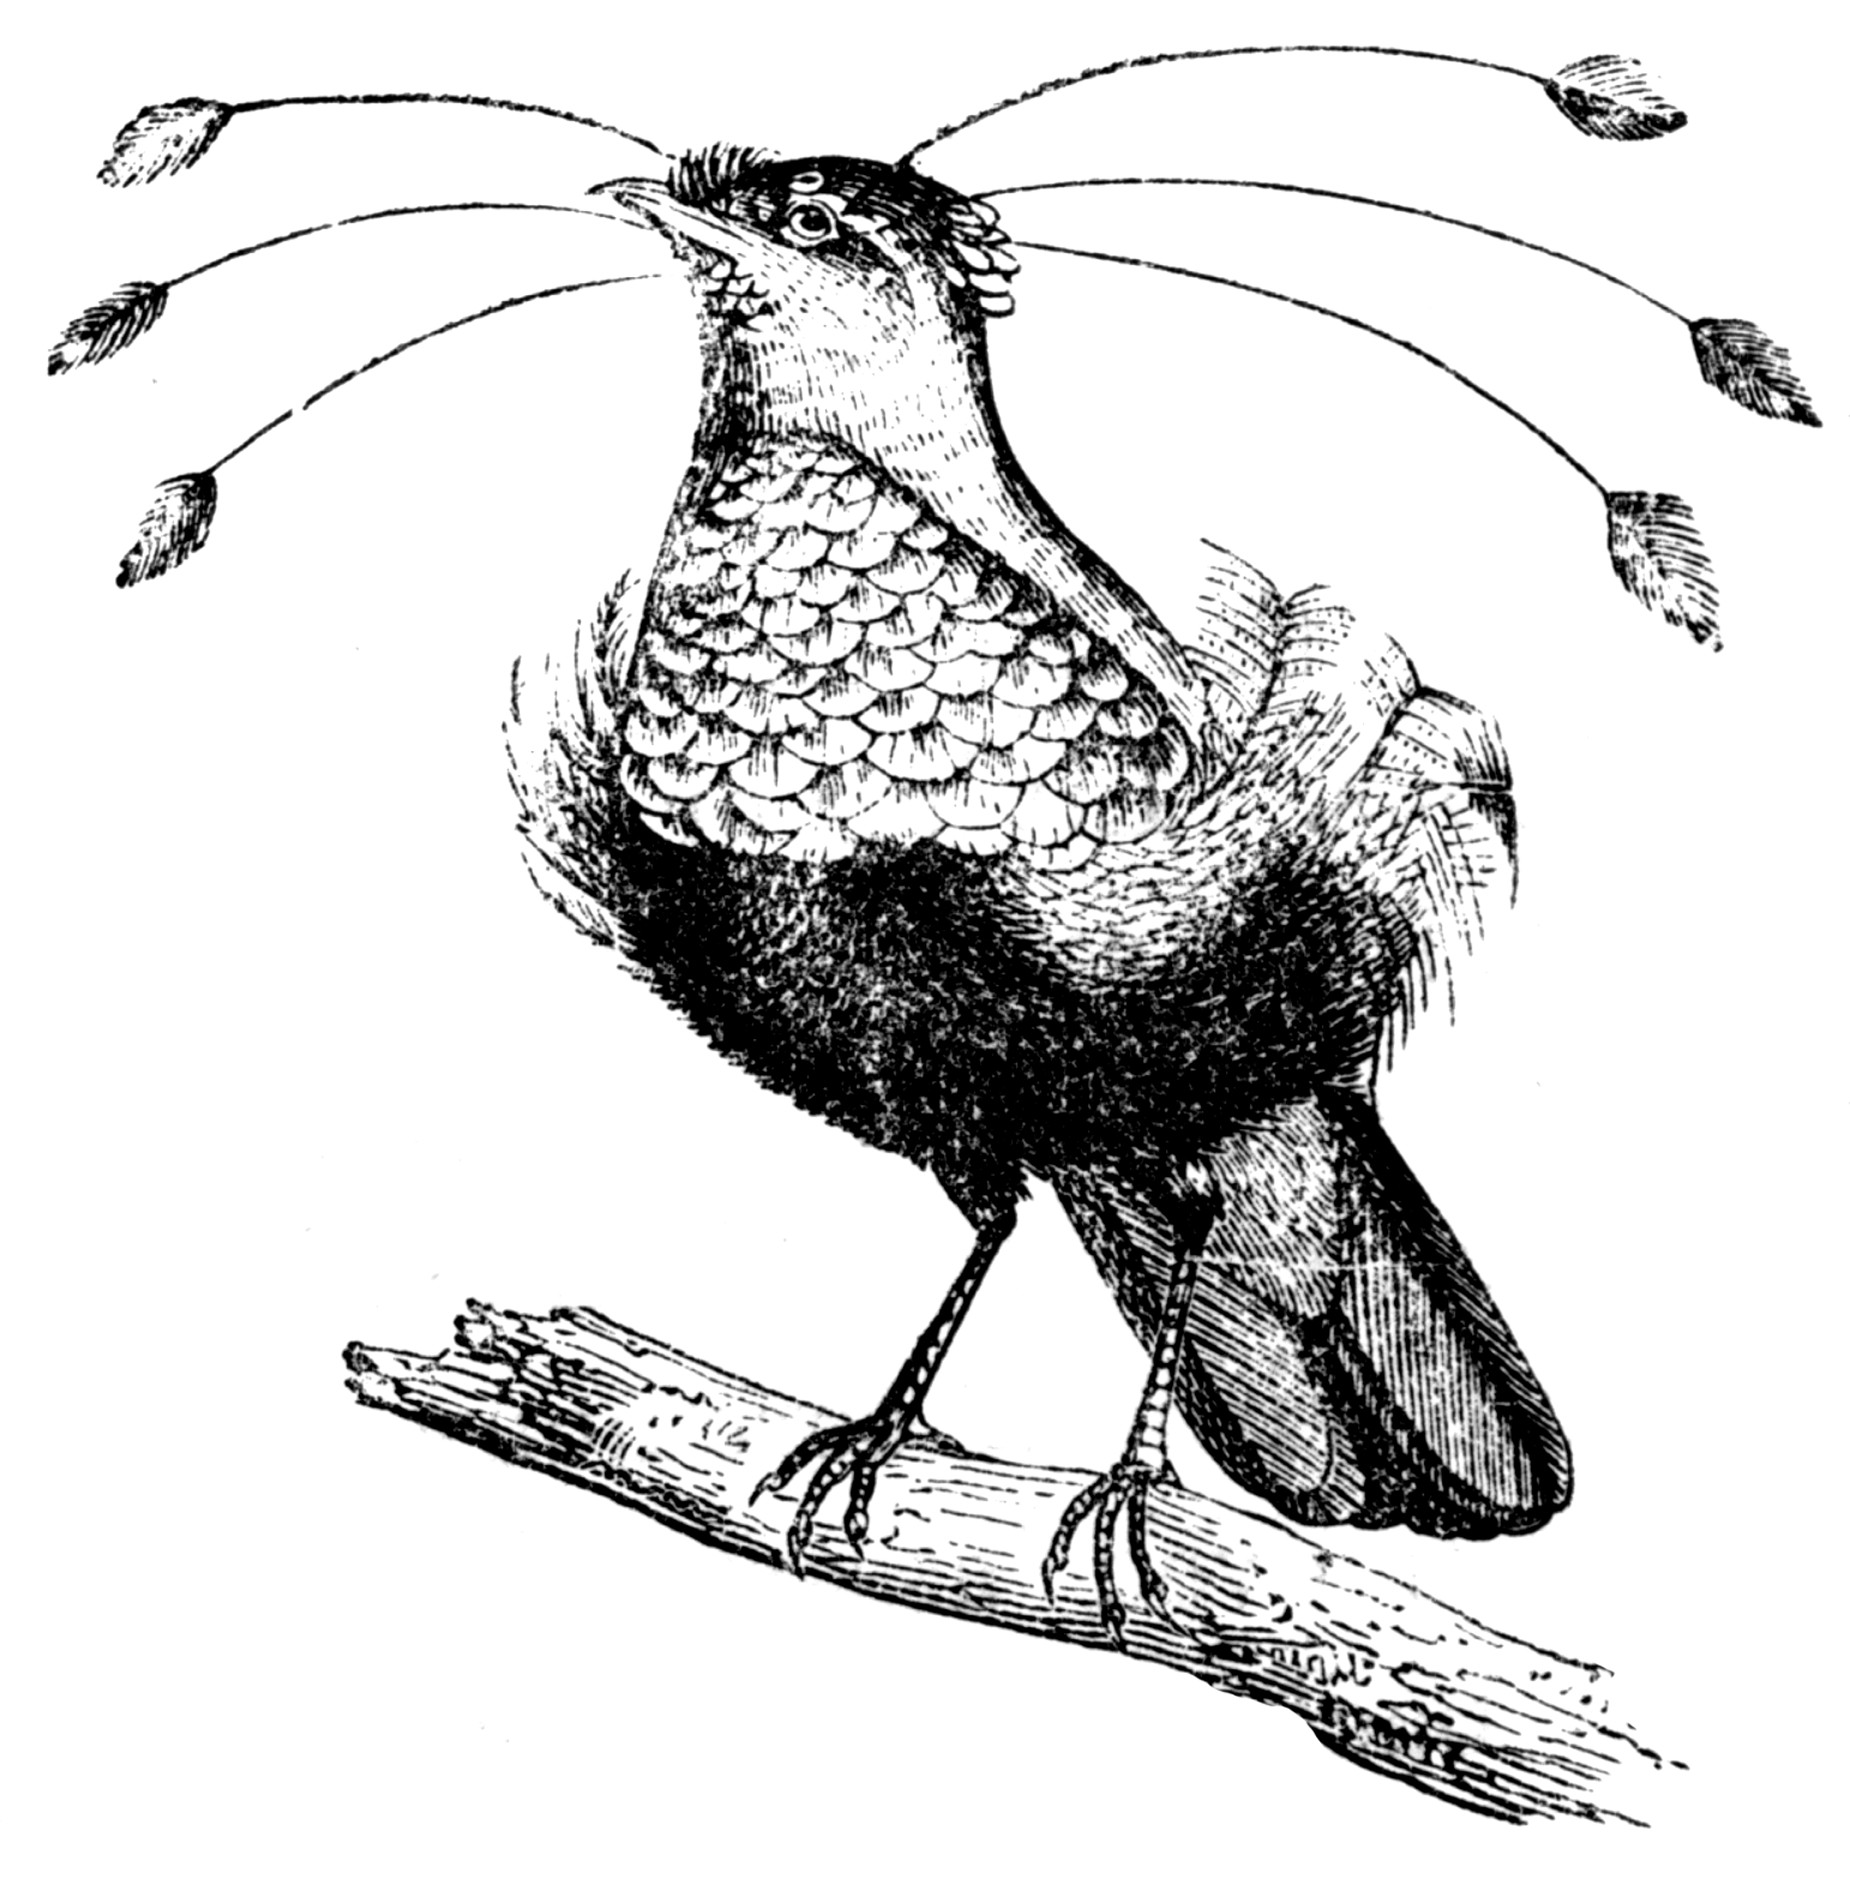
\includegraphics[width=0.3\textwidth]{paradise.png}
	}
	\caption{Louis Figuier, ``Reptiles and Birds'', 1869. This artwork symbolizes the adversarial relationship in game theory, where different entities compete for dominance, much like the generator and discriminator in GANs.}
\end{figure}
\vspace{0.5cm}
The Generative Adversarial Network (GAN) framework is fundamentally rooted in game theory, which studies strategic interactions between rational decision-makers using mathematical models~\cite{ref:myerson}. In this section, we examine GANs through the lens of two-player games, where the discriminator ($D$) and generator ($G$) engage in an adversarial competition. We denote their value functions as $V_D$ and $V_G$, respectively.
\subsection{Game-Theoretic Foundations}
\begin{definition}%
	\label{def:value-function}
	A \textnormal{\sffamily value function} $V_i$ quantifies the reward (or loss if negative) for player $i$ in a game, expressed as a function of the player's actions.
\end{definition}
\begin{remark}
	In many machine learning contexts, the loss function represents the difference between target values $y$ and estimates $\hat{y}$. In GANs, however, the value function is more complex, serving as a measure of uncertainty in the adversarial game.
\end{remark}
The original GAN formulation~\cite{ref:goodfellow-original} introduces two value functions. The first frames GANs as a zero-sum game, while the second provides a more practical training objective~\cite{ref:gidel-variational-2018}.
\begin{definition}%
	\label{def:zero-sum-game}
	A \textnormal{\sffamily zero-sum game} is one where one player's gain exactly equals the other player's loss. Formally, $V_D + V_G = 0$.
\end{definition}
\begin{remark}
	For this section, we focus on the zero-sum formulation, where the GAN algorithm represents a strategic competition between the generator and discriminator (see Definitions~\ref{def:generator} and~\ref{def:discriminator}).
\end{remark}
\subsection{Minimax Strategy and Equilibrium}
In zero-sum games, players seek optimal strategies to maximize their minimum possible reward. The minimax decision rule provides a framework for this optimization.
\begin{definition}
	\label{def:minimax}
	In a two-player game with players $D$ and $G$, the \textnormal{\sffamily minimax decision rule} for $D$ maximizes $D$'s expected reward after $G$ has minimized $D$'s maximum attainable reward. The \textnormal{\sffamily minimax value} $\overline{V_D}$ is:
	\begin{align}
		\overline{V_D} = \min_{G} \max_{D} V_D(D, G).
	\end{align}
\end{definition}
The minimax strategy ensures the best possible outcome against an optimal opponent. If $G$ moves first to minimize $D$'s reward, $D$'s minimax rule maximizes the reduced reward.
\subsection{Nash Equilibrium and Strategic Stability}
The GAN algorithm seeks a Nash equilibrium in the parameter space of the discriminator and generator~\cite{ref:goodfellow-2016,ref:goodfellow-2017}.
\begin{definition}
	A \textnormal{\sffamily Nash equilibrium} in an $n$-player game is a strategy profile $s^* = (s_1, s_2, \dots, s_n)$ where no player can benefit by unilaterally changing their strategy. Formally, for all players $i$ and alternative strategies $s_{-i}$:
	\begin{align}
		f_i(s^*) \geq f_i(s_1, s_2, \dots, s_{-i}, \dots, s_n)
	\end{align}
	where $f_i(s)$ is the payoff to player $i$ under strategy profile $s$.
\end{definition}
\begin{remark}
	In a Nash equilibrium, each player's strategy is optimal given the others' strategies. For zero-sum games, the minimax solution corresponds to a Nash equilibrium. Note that Nash equilibria are not necessarily globally optimal, and multiple equilibria may exist.
\end{remark}
\subsubsection{Prisoner's Dilemma: A Case Study}
\label{sec:prisoners-dilemma}
The Prisoner's Dilemma illustrates key concepts of Nash equilibrium and strategic interaction. Originally formulated by Flood and Dresher in the 1950s and later reformulated by Tucker~\cite{ref:poundstone}, it demonstrates how individual rationality can lead to suboptimal collective outcomes.
In this game, two players ($D$ and $G$) are held in separate custody with no communication. Each faces the following choices:
\begin{enumerate}
	\item If one defects (accuses the other) while the other denies, the defector receives 1 year (reward for cooperation) while the other receives 5 years.
	\item If both deny, each receives 2 years (sufficient evidence exists for the lesser crime).
	\item If both defect, each receives 3 years.
\end{enumerate}
\begin{figure}[h]
	\centering%
	\bgroup%
	\def\arraystretch{1.4}
	\begin{tabular}[c]{|c|c|c|}
		\hline
		\diagbox{$D$}{$G$} & Deny   & Defect \\
		\hline
		Deny               & (2, 2) & (5, 1) \\
		\hline
		Defect             & (1, 5) & (3, 3) \\
		\hline
	\end{tabular}
	\egroup
	\caption{Prisoner's Dilemma payoff matrix (years in prison for $D$, $G$). The global optimum (Deny, Deny) is unstable, while (Defect, Defect) is the Nash equilibrium.}%
	\label{fig:prisoners-matrix}
\end{figure}
Analyzing all possible states:
\begin{enumerate}
	\item \textbf{(Deny, Defect)}: If $D$ switches to defect while $G$ defects, $D$ improves from 5 to 3 years. This is not a Nash equilibrium (and symmetrically for (Defect, Deny)).
	\item \textbf{(Deny, Deny)}: If $D$ switches to defect while $G$ denies, $D$ improves from 2 to 1 year. This is not a Nash equilibrium.
	\item \textbf{(Defect, Defect)}: Neither player can improve by unilaterally changing strategy. If $D$ switches to deny while $G$ defects, $D$ worsens from 3 to 5 years. This is the Nash equilibrium.
\end{enumerate}
This example shows that the globally optimal outcome (Deny, Deny) is unstable, while the Nash equilibrium (Defect, Defect) is stable but suboptimal. This has important implications for GANs, as we'll see later.
\subsection{Derivation of the GAN Value Function}%
\label{sec:derivation}
We now derive the GAN value function from game-theoretic principles. Let $(\mathcal{X}, p_{data})$ be a probability space where $\mathcal{X}$ is a finite space (e.g., the space of all $H \times W$ 8-bit RGB images, $\mathcal{X} = [0, 255]^{3 \times H \times W}$) and $p_{data}$ assigns mass to regions corresponding to meaningful images.
The GAN algorithm trains a generator $G_\phi$ (parameterized by $\phi \in \Phi \subset \mathbb{R}^n$) to map random samples $z$ from a prior space $(\mathcal{Z}, p_z)$ to $\mathcal{X}$ such that $G_\phi(z)$ lies in regions where $p_{data}$ assigns significant mass. Typically, $\mathcal{Z} \neq \mathcal{X}$ and $|\mathcal{Z}| < |\mathcal{X}|$~\cite{ref:arjovsky-2017}.
\begin{figure}[H]
	\centering
	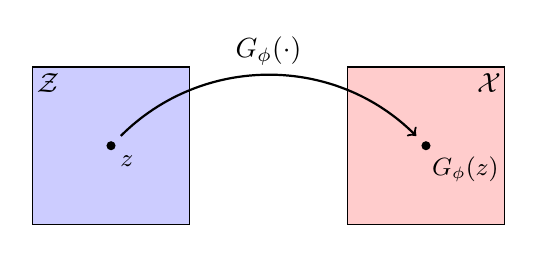
\begin{tikzpicture}
		\node (G) at (3, 2.2) {$G_\phi(\cdot)$};
		\draw[fill=blue!20] (0, 0) rectangle +(2, 2);
		\node at (0.2, 1.8) {$\mathcal{Z}$};
		\filldraw (1, 1) circle (0.05cm);
		\node (Z) at (1, 1) {};
		\node (ZZ) at (1.2, 0.8) {\small $z$};
		\draw[fill=red!20] (4, 0) rectangle +(2, 2);
		\filldraw (5, 1) circle (0.05cm);
		\node (O) at (5, 1) {};
		\node (OO) at (5.5, 0.7) {\small $G_\phi(z)$};
		\node at (5.8, 1.8) {$\mathcal{X}$};
		\draw[->,thick] (Z) to [out=45,in=135] (O);
	\end{tikzpicture}
	\caption{The generator $G_\phi$ transforms noise $z \sim p_z$ into synthetic samples $G_\phi(z) \in \mathcal{X}$. The goal is for these samples to lie in high-probability regions under $p_{data}$.}%
	\label{fig:g-maps}
\end{figure}
Initially, $G_\phi$ maps $z$ to $\mathcal{X}$ randomly. Through adversarial training, both $D_\theta$ and $G_\phi$ learn $p_{data}$ from different perspectives: $D_\theta$ learns to distinguish real from generated samples, while $G_\phi$ learns to generate samples that fool $D_\theta$.
The value function $V$ captures this adversarial dynamic:
\begin{align}
	\label{eq:the-original-objective-function}
	V(D_\theta, G_\phi) = \mathbb{E}_{x \sim p_{data}}[\log D_\theta(x)] + \mathbb{E}_{z \sim p_z}[\log(1 - D_\theta(G_\phi(z)))].
\end{align}
This value function resembles the noise-contrastive estimator~\cite{ref:gutmann-2010}. In the game between $G_\phi$ and $D_\theta$, each seeks to maximize their minimum reward by playing their minimax decision rule.
\subsubsection{Discriminator's Objective}%
\label{sec:derivation-d}
From $D_\theta$'s perspective, we want $D_\theta(x)$ to approximate $p_{data}(x)$. We find $\theta \in \Theta$ that maximizes the likelihood:
\begin{align}
	\label{eq:d-1}
	L_D^{(1)}(\theta) = \prod_{i=1}^n D_\theta(x_i), \quad x_i \sim p_{data}.
\end{align}
For numerical optimization, we maximize the log-likelihood:
\begin{align}
	\label{eq:d-l1}
	\ell_D^{(1)}(\theta) = \sum_{i=1}^n \log D_\theta(x_i).
\end{align}
Simultaneously, $D_\theta$ must assign low probability to generated samples $G_\phi(z) = \tilde{x}$. For fixed $G_\phi$, $\theta$ should minimize:
\begin{align}
	L_D^{(2)}(\theta) = \prod_{i=1}^n D_\theta(G_\phi(z_i)), \quad z_i \sim p_z.
\end{align}
Equivalently, we minimize the log-likelihood:
\begin{align}
	\label{eq:d-l2} \ell_D^{(2)}(\theta) = \sum_{i=1}^n \log D_\theta(G_\phi(z_i)).
\end{align}
To combine both objectives, we maximize the complement:
\begin{align}
	\ell_D^{(2)}(\theta) = \sum_{i=1}^n \log(1 - D_\theta(G_\phi(z_i))),
\end{align}
since minimizing $D_\theta(G_\phi(z))$ is equivalent to maximizing $1 - D_\theta(G_\phi(z))$. Combining both objectives, $D_\theta$ maximizes:
\begin{align}
	\sum_{i=1}^n \left( \log D_\theta(x_i) + \log(1 - D_\theta(G_\phi(z_i))) \right).
\end{align}
By the law of large numbers, this sample average converges to:
\begin{align}
	\label{eq:objective-for-d}
	\mathbb{E}_{x \sim p_{data}}[\log D_\theta(x)] + \mathbb{E}_{z \sim p_z}[\log(1 - D_\theta(G_\phi(z)))]
\end{align}
for sufficiently large $n$.
\subsubsection{Generator's Objective}%
\label{sec:derivation-g}
From $G_\phi$'s perspective, we seek $\phi$ that maximizes the likelihood (as judged by a fixed $D_\theta$) that generated samples come from $p_{data}$. We maximize:
\begin{align}
	\ell_G(\phi) = \sum_{i=1}^n \log D_\theta(G_\phi(z_i)), \quad z_i \sim p_z.
\end{align}
Equivalently, we minimize:
\begin{align}
	\ell_G(\phi) = \sum_{i=1}^n \log(1 - D_\theta(G_\phi(z_i))),
\end{align}
which corresponds to minimizing $\mathbb{E}_{z \sim p_z}[\log(1 - D_\theta(G_\phi(z)))]$.
\subsubsection{Minimax Formulation}
The training objectives lead to the minimax formulation:
\begin{align}
	\overline{V_D} & = \min_{\phi}\max_{\theta} V_D(\theta, \phi)                                                                                                      \\
	               & = \min_{\phi}\max_{\theta} \left( \mathbb{E}_{x \sim p_{data}}[\log D_\theta(x)] + \mathbb{E}_{z \sim p_z}[\log(1 - D_\theta(G_\phi(z)))] \right)
\end{align}
We solve this by finding the minimax decision rule and value for $D_\theta$ (Theorem~\ref{theorem:minimax}), which corresponds to the Nash equilibrium. However, finding this equilibrium is often challenging in practice.
\subsection{Challenges in Finding Nash Equilibrium}%
\label{sec:difficulty}
Finding Nash equilibria can be difficult, as demonstrated by the following example inspired by~\cite{ref:weng-2017}:
\begin{example}[Oscillatory Dynamics]
	Let $V(x, y) = xy$ be a value function with the game:
	\begin{align}
		\min_x \max_y V(x, y) = xy.
	\end{align}
	The gradients are $\frac{\partial V}{\partial x} = y$ and $\frac{\partial V}{\partial y} = x$, leading to updates:
	\begin{align}
		x^{(t+1)} & \gets x^{(t)} - \eta \cdot y, \\
		y^{(t+1)} & \gets y^{(t)} + \eta \cdot x,
	\end{align}
	where $\eta > 0$ is the learning rate.
	The Nash equilibrium is $s^* = (s_G^*, s_D^*) = (0, 0, \dots)$, where $V(s_G^*, s_D) = 0$ for all $s_D$, and $V(s_G, s_D^*) = 0$ for all $s_G$.
	\begin{figure}[H]
		\centering
		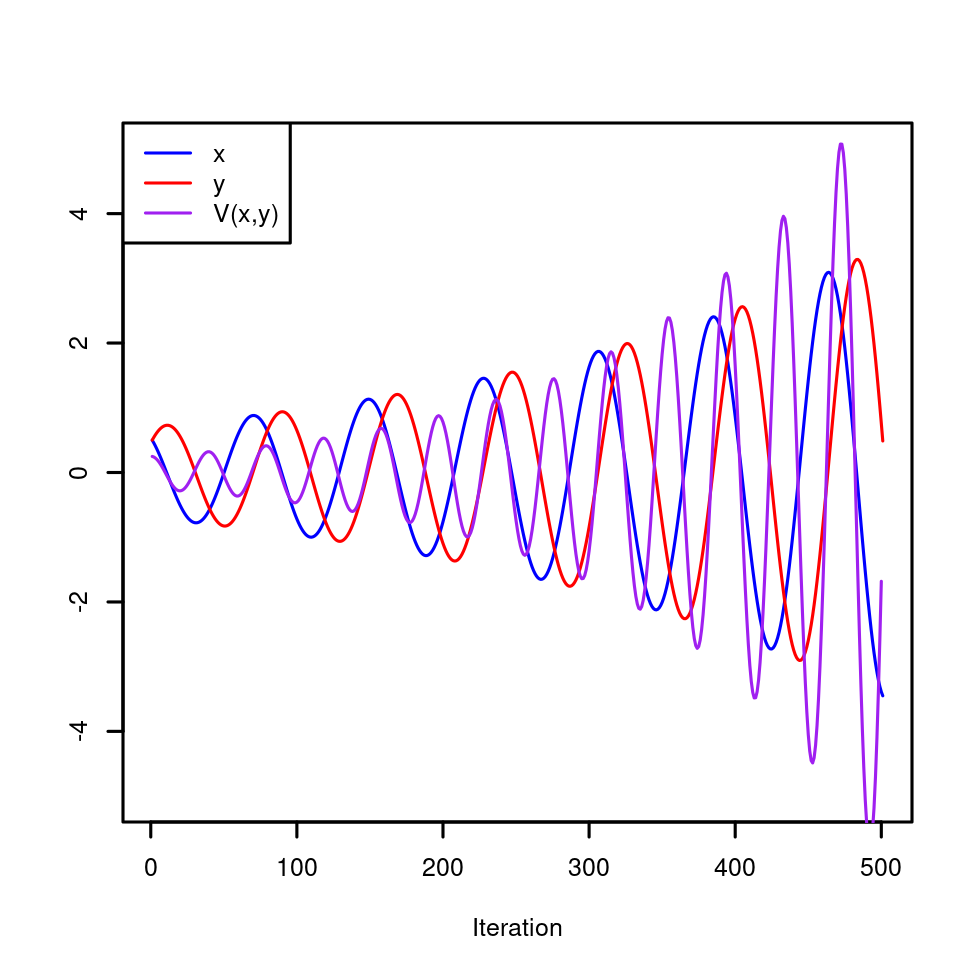
\includegraphics[width=0.6\textwidth]{plot1.png}
		\caption{Oscillatory behavior around the Nash equilibrium. This pattern is commonly observed in GAN training, where generator and discriminator parameters oscillate rather than converging to a stable equilibrium.}%
		\label{fig:alternating}
	\end{figure}
\end{example}
This oscillatory behavior is frequently observed in GAN training, where alternating gradient updates can cause the system to oscillate around equilibrium rather than converge to it.
\subsection{Alternative Value Functions}%
\label{sec:two-value}
The original value function (Equation~\ref{eq:the-original-objective-function}) often leads to vanishing gradients, especially early in training when $D_\theta$ easily distinguishes real from generated samples. To address this,~\cite{ref:goodfellow-original} introduced an alternative formulation:
\begin{align}
	\label{eq:second-value-function}
	\max_{\theta} \left( \mathbb{E}_{x \sim p_{data}}[\log D_\theta(x)] + \mathbb{E}_{z \sim p_z}[\log(1 - D_\theta(G_\phi(z)))] \right) \\
	\max_{\phi} \mathbb{E}_{z \sim p_z}[\log D_\theta(G_\phi(z))]
\end{align}
These decoupled objectives share the same fixed points as the original formulation but provide stronger gradients for the generator, improving learning dynamics. With this formulation, GANs are no longer strictly zero-sum games.
\subsection{GAN Algorithm}
The complete GAN algorithm is presented below:
\begin{figure}[H] \centering
	\begin{minipage}{0.95\linewidth}
		\begin{algorithm}[H]
			\SetAlgoLined
			\KwIn{Learning rate $\eta > 0$, Number of iterations $T > 0$}
			\KwOut{Trained discriminator $D_\theta$ and generator $G_\phi$}
			Initialize discriminator parameters $\theta$ and generator parameters $\phi$ randomly\;
			\For{$t = 1$ \KwTo $T$}{
				\textbf{// Update discriminator}\;
				Sample batch $\{x_1, \dots, x_m\}$ from real data distribution $p_{data}$\;
				Sample batch $\{z_1, \dots, z_m\}$ from prior noise distribution $p_z$\;
				Compute discriminator loss:
				\[
					L_D = -\frac{1}{m} \sum_{i=1}^m \left[ \log D_\theta(x_i) + \log(1 - D_\theta(G_\phi(z_i))) \right]
				\]
				Update discriminator parameters: $\theta \gets \theta - \eta \cdot \nabla_\theta L_D$\;
				\textbf{// Update generator}\;
				Sample batch $\{z_1, \dots, z_m\}$ from prior noise distribution $p_z$\;
				Compute generator loss:
				\[
					L_G = -\frac{1}{m} \sum_{i=1}^m \log D_\theta(G_\phi(z_i))
				\]
				Update generator parameters: $\phi \gets \phi - \eta \cdot \nabla_\phi L_G$\;
			}
			\caption{Generative Adversarial Networks Algorithm}
			\label{algo:main-algo}
		\end{algorithm}
	\end{minipage}
\end{figure}
Note that in the original paper, the discriminator is updated $k$ times per generator update (typically $k=1$). We've omitted this inner loop for clarity, but it can be important for stability in practice.
\subsection{Strategic Interpretation and Discussion}
The minimax strategy for $D_\theta$ has an important interpretation: if $D_\theta$ assumes $G_\phi$ has done its worst (i.e., generated perfect samples), then $D_\theta$ should assign probability $1/2$ to all inputs. This is the maximum entropy distribution over the two states (real or synthetic), representing maximum uncertainty.
When $D_\theta(x) = 1/2$ for all $x$, the generator receives no useful gradient signal and cannot improve. This represents a strategic equilibrium where neither player can benefit by unilaterally changing their strategy. In the next section, we'll show that $D_\theta(x) = 1/2$ is indeed the optimal strategy for $D_\theta$ at equilibrium.
This game-theoretic perspective reveals fundamental challenges in GAN training:
\begin{itemize}
	\item The minimax formulation can lead to oscillatory dynamics rather than stable convergence
	\item The zero-sum assumption may not hold in practice, as both networks ultimately benefit from reaching a good equilibrium
	\item Alternative value functions can improve training stability by providing better gradient signals
\end{itemize}
Understanding these strategic dynamics is crucial for developing improved GAN variants and training procedures, as we'll explore in subsequent sections.
%%% Local Variables:
%%% mode: latex
%%% TeX-master: "../thesis.tex"
%%% End:
